\section{ارجاع‌دهی‌‌ها}
\begin{frame}{ارجاع‌دهی‌‌ها در خود سند}
\begin{itemize}\itemr
\item[-]
در مواقع زیادی نیاز به ارجاع‌دهی در قسمت‌ها مختلف سند، احساس می‌شود.
\item[-]
برای مثال برای ارجاع‌دهی به یک فصل خاص، سکشن‌ خاص، جدول و یا تصاویر مختلف نیاز به یک ارجاع‌دهی پویا داریم.

\item[-]
فرض کنید چنین متنی داریم: \textit{با توجه به مباحثی که در فصل ۲ انجام شد...}
و سپس تصمیم می‌گیریم که قبل از فصل ۲، یک فصل دیگر بنویسیم و در واقع فصل ۲، می‌شود فصل ۳.

\item[-]
اگر این ارجاع‌دهی را به صورت دستی انجام داده باشیم، باید بگردیم و تمامی \textit{فصل ۲}‌های داخل متنمان را به \textit{فصل ۳} تغییر بدهیم.

\item[-]
اما، همانند کاری که برای شمارنده‌ها کردیم، میتوانیم از امکانات خود لاتک برای ارجاع‌دهی استفاده کنیم.
\end{itemize}
\end{frame}

\begin{frame}{ارجاع‌دهی‌‌ها در خود سند}
\begin{itemize}\itemr
\item[-]
برای اینکار باید از دو دستور استفاده کنیم:
\begin{enumerate}\itemr
\item 
\lr{\texttt{\textbackslash lable\{UniqueLabel\}}} 
برای نشانه‌گذاری

\item 
\lr{\texttt{\textbackslash ref\{UniqueLable\}}}
برای ارجاع‌دهی 
\end{enumerate}
\end{itemize}
\end{frame}

\begin{frame}[fragile]{نمونه کد}
\begin{latin}
\begin{lstlisting}[keywords={chapter, section, label, ref}, keywordstyle=\color{Mulberry}\textbf]
\chapter{Processes and Threads}
\section{Processes}\label{processes}
\section{Threads}
As mentioned in the \ref{processes},
OS must schedule and dispatch...
\end{lstlisting}
\end{latin}
\end{frame}

\begin{frame}{خروجی}
\begin{center}
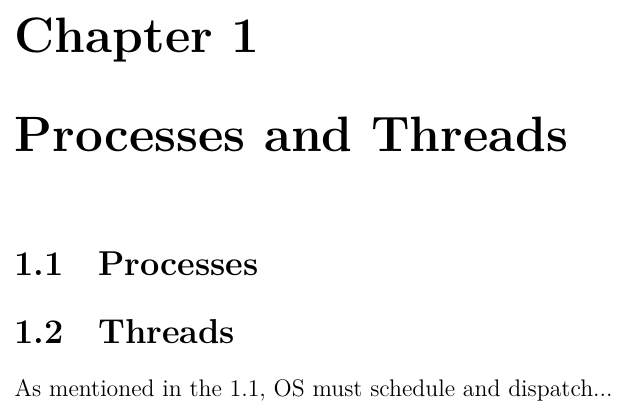
\includegraphics[width=0.65\textwidth, height=0.7\textheight]{docs/images/proc-ref}
\end{center}
\end{frame}


\begin{frame}[fragile]{نمونه کد}
\begin{latin}
\begin{lstlisting}[keywords={chapter, section, label, ref}, keywordstyle=\color{Mulberry}\textbf]
\chapter{Processes and Threads}
\section{Operating System}
\section{Processes}\label{processes}
\section{Threads}
As mentioned in the \ref{processes}, 
OS must schedule and dispatch...
\end{lstlisting}
\end{latin}
\end{frame}

\begin{frame}{خروجی}
\begin{center}
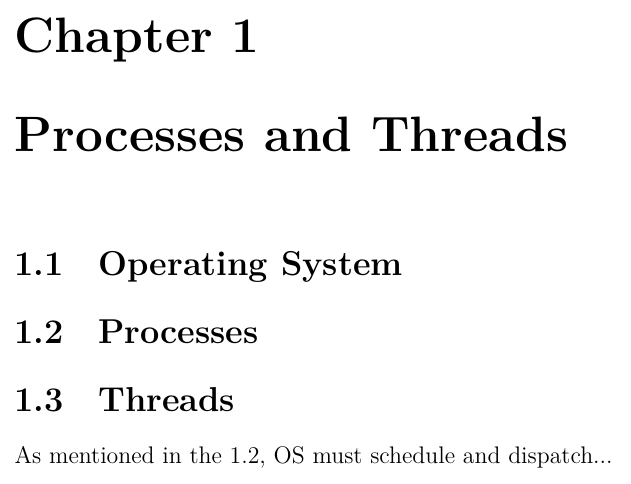
\includegraphics[width=0.55\textwidth, height=0.7\textheight]{docs/images/proc-ref-1}
\end{center}
\end{frame}

\begin{frame}{ارجاع‌دهی‌‌ها در خود سند}
\begin{itemize}\itemr
\item[-]
حتی می‌توان بجای ارجاع‌دهی با عدد، با نام هم به مطلب مورد نظر، ارجاع داد.

\item[-]
برای این کار باید از بسته‌ی 
\lr{\texttt{nameref}}
و تگ
\lr{\texttt{\textbackslash nameref\{UniqueLable\}}}
استفاده کرد.
\end{itemize}
\end{frame}

\begin{frame}[fragile]{نمونه کد}
\begin{latin}
\begin{lstlisting}[keywords={chapter, section, label, ref}, keywordstyle=\color{Mulberry}\textbf]
\chapter{Processes and Threads}
\section{Processes}\label{processes}
\section{Threads}
As mentioned in the \nameref{processes},
OS must schedule and dispatch...
\end{lstlisting}
\end{latin}
\end{frame}

\begin{frame}{خروجی}
\begin{center}
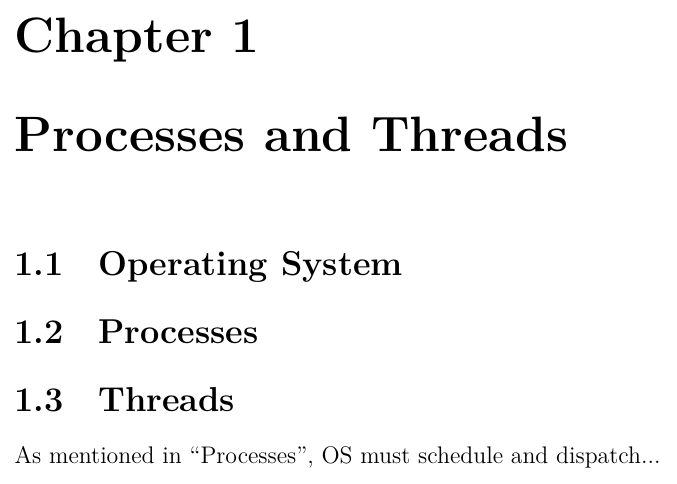
\includegraphics[width=0.55\textwidth, height=0.7\textheight]{docs/images/proc-nameref}
\end{center}
\end{frame}

\begin{frame}[fragile]{نمونه کد}
\begin{latin}
\begin{lstlisting}[keywords={chapter, section, label, ref}, keywordstyle=\color{Mulberry}\textbf]
\chapter{Processes and Threads}
\section{What Are Processes?}\label{processes}
\section{Threads}
As mentioned in the \nameref{processes},
OS must schedule and dispatch...
\end{lstlisting}
\end{latin}
\end{frame}

\begin{frame}{خروجی}
\begin{center}
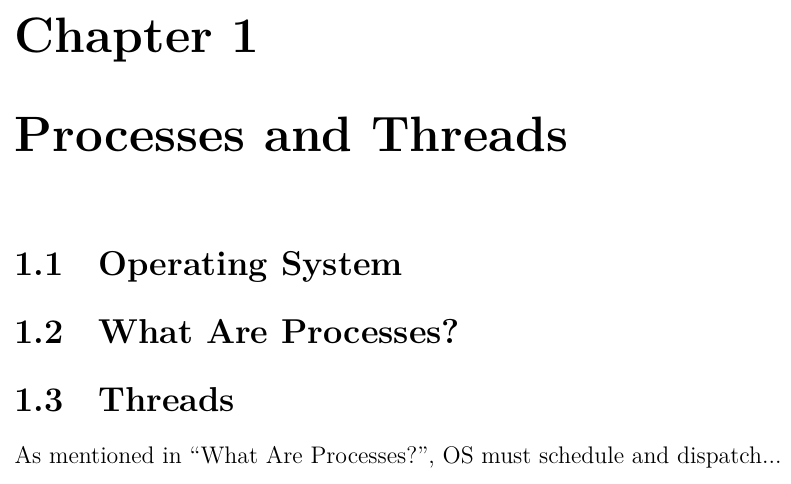
\includegraphics[width=0.7\textwidth, height=0.75\textheight]{docs/images/proc-nameref-change}
\end{center}
\end{frame}
